

\documentclass[12pt,svgnames,smaller]{article} % use larger type; default would be 10pt

\usepackage[table]{xcolor}
\usepackage[utf8]{inputenc} % set input encoding (not needed with XeLaTeX)
\usepackage[pdftex]{graphicx}

\usepackage{geometry} % to change the page dimensions
\geometry{a4paper} % or letterpaper (US) or a5paper or....

\usepackage{graphicx} % support the \includegraphics command and options

\usepackage[parfill]{parskip} % Activate to begin paragraphs with an empty line rather than an indent

\usepackage{verbatim} % adds environment for commenting out blocks of text & for better verbatim
\usepackage{mathrsfs}

\usepackage{amssymb}
\usepackage{amsthm}
\newtheorem{myalg}{Algorithm}
\newtheorem{mydef}{Definition}
\newtheorem{myprop}{Proposition}
\newtheorem{myproof}{Proof}
\newtheorem{myexample}{Example}

\usepackage{amsmath}
\newcommand{\E}[1]{\textnormal{\textsf{E}}\!\left[#1\right]} % expectation

\usepackage{tabularx}

%\usepackage{tabulary}

\renewcommand{\labelenumi}{\alph{enumi})} % change the listing of the enumerations to a) b) c)

\renewcommand{\labelenumii}{\roman{enumii}.} % change the listing of the second level of lists to i. ii. iii.

\newenvironment{xitemize}
	{\begin{minipage}[t]{0.5\textwidth}\begin{itemize}}
	{\end{itemize}\end{minipage}}

\begin{document}
\begin{titlepage}
\begin{center}

% Upper part of the page
% ======================

\textsc{\large Jomo Kenyatta University of Agriculture and Technology (JKUAT)}\\[0.4cm]
%\textsc{\Large College of Pure and Applied Science (COPES)}\\[1.0cm]
%\textsc{\Large School of Computing and Information Technology (SCIT)}\\[0.5cm]
\textsc{\large Department of Computing}\\[0.4cm]
\textsc{\large ICS2406: Computer Systems Project  }\\[0.3cm]
\textsc{\large Draft Project Proposal }\\[0.3cm]
\textsc{\large REF:JKU/2/83/022 }\\[0.2 cm]

% Title
% =====
 
\begin{figure}
	\centering
	\includegraphics[width=0.7\linewidth]{"/run/media/joshua/DATA/ICS_2406_Pictures/Base/JKUAT_Logo"}
	\label{fig:JKUAT_logo}
\end{figure}
\textbf{\texttt{ Exchange Of Audio Information Via Wireless Technology}}{\vspace*{20 mm}}
\end{center}

% Author and supervisors
% ======================

\begin{figure}
	\centering
	\includegraphics[width=0.7\linewidth]{/run/media/joshua/DATA/ICS_2406_Pictures/Base/JKUAT_Logo}
	\label{fig:JKUAT_logo}
\end{figure}


\begin{minipage}{1.0\textwidth}	
	\begin{flushleft} \large
		\emph{Author:}\\
		Name: Kairu \textsc{Joshua Wambugu} Reg. No: CS281-0720/2011 \\
		Submission Date: \hrulefill  Sign: \hrulefill \\
		Course: Bsc. Computer Science
	\end{flushleft}
\end{minipage}

\begin{minipage}{1.0\textwidth}
	\begin{flushleft} \large
		\emph{Supervisor 1:} \\
		Name: \hrulefill Sign: \hrulefill Date: \hrulefill
		%John Masika \textsc{Masinde}
	\end{flushleft}
\end{minipage}

\begin{minipage}{1.0\textwidth}
	\begin{flushleft} \large
		\emph{Supervisor 2:} \\
		Name: \hrulefill Sign: \hrulefill Date: \hrulefill
		%John Kevin \textsc{Otieno}
	\end{flushleft}
\end{minipage}

\begin{minipage}{1.0\textwidth}
	\begin{flushleft} \large
		\emph{Supervisor 3:} \\
		Name: \hrulefill Sign: \hrulefill Date: \hrulefill
		%Jane Claire \textsc{Mwaura}
	\end{flushleft}
\end{minipage}

\vfill

% Bottom of the page
% ==================

\begin{center}
	{\large Period: June 2015}
\end{center}
%{\large \today}
%\end{center}
\end{titlepage}

%\maketitle

% begin Preface
% ============

\textbf{Preface}

Have you ever been in a situation where you are in close proximity – maybe only separated by a wall - to someone you want to talk with but still have to use airtime to converse with them? At one time or another we face this challenge. It can be rather frustrating. But with all the power we have in our pockets in the form of intelligent smart phones, should this really be a problem? Should not technology let us solve this small annoyances so that we can focus on bigger problems such as climate change and space exploration? Questions such as these are what gave rise to this project. Will it be possible to connect smart phones over about 100 metres without using airtime? Let us see.

% end Preface
% ==========

\clearpage

% begin Acknowledgements
% =======================

\textbf{Acknowledgements}

I would wish to take the next few lines of text to acknowledge the individuals who have made it possible for me to finish this project.

% begin itemize acknowledgements
\begin{itemize}
	\item Jehovah God, the true God, the Creator and the Maintainer of the Universe, for giving me the wisdom, the courage, the supportive environment and the opportunity to finish this project.
	\item My parents, Hosea Kairu Wambugu and Joyce Njoki Kairu, for sharing their experiences, giving words of wisdom, and always pushing me when I became slightly lazy.
	\item The project coordinator, Harriet Ratemo, setting the infrastructure needed for my project mates and I to go through the project process without worrying about technical details outside the project's scope.
	\item My supervisors Professor Waweru Mwangi and Doctor Petronilla Muriithi for providing invaluable advice on, among other things, how to present my project in an acceptable manner.
	\item Julian Keya for assisting me do the experiments whose results are presented in this project.
\end{itemize}
% end itemize acknowledgements

\clearpage

% end Acknowledgements
% ======================

% begin Abstract
% =============

\textbf{Abstract}

This project is an effort to reduce cost. One of the ways we incur expenses in our daily lives is through communication. Specifically, communicating through a third party increases costs since it calls for compensation of that third entity. Removing the third party during communication would reduce communication costs substantially. The most common communication devices among humanity at the moment are mobile phones. And smart phones will be just as common very soon. For individuals to contact each other via smartphones, a third party – such as a carrier – is usually involved. While there are many ways to remove this third party, the project to follow will focus on establishing an audio communication between two smartphones over a wireless connection without a third party. It is hoped that the idea behind this project will, in the (probably very) long run reduce communication costs between owners of smart devices. 

\clearpage

% end Abstract
% ===========

\tableofcontents
\clearpage

% begin Background/Introduction
% =============================

\section{ \textbf{ Background/Introduction } }
 
	The 21st Century has been characterised by very fast developments in technology. Services that we thought were impossible 100 or even 50 years ago are now commonplace, resulting in a lot of expediency. Among the devices that have brought this convenience – or inconvenience depending on one’s viewpoint – is the mobile phone.

	The mobile phone technology allows people to use handheld telephones to communicate with others despite the physical distance between them. This communication is done either via voice by one user calling another; or via reading by one user sending another a message using the Short Message Service (SMS). Both of these forms of communication usually involve the user having to pay the network service provider some money in exchange for the use of the provider’s infrastructure to call or SMS.  For the most part, the payment to the network provider outweighs the cost and inconvenience of a cell phone user having to set up their own equipment so as to achieve the same communication. But what if the two users were just a few meters away, maybe just separated by a wall? Would it make sense to have to pay the network service provider to communicate with someone so near? For quite some time, it seemed that mobile phone users had no choice.
	
	Within the past half-decade or so, cellular phones have grown from just being devices to send and receive voice and SMS data to being devices that can do much more. Smartphones – loosely defined as cell phones with computer capabilities – have given people the capability to not only call and text but also check their email, surf the Internet, listen to music, keep up to date with the latest news, just to mention a few things. Smartphones have revolutionised the mobile phone revolution. With this mind, consider: It is currently possible for two networked computers to send and receive not only audio but also video data between themselves via a process known as streaming. The network between the two computers could either be wired or wireless. Could the same streaming be done between smartphones? A “Yes” answer with the corresponding implementation could conveniently put the network service provider out of the picture. And that question dovetails nicely into this project’s problem statement.

% end Background/Introduction
% =============================

% begin Problem Statement
% =======================

\section{ \textbf{ Problem Statement } } 

The research question that will guide this project is:

\textbf{ How can smartphones communicate with each other over short distances without incurring network service provider costs? }

By the end of this project, the following objectives should have been met:

% list of objectives
\begin{itemize}
	\item Two smartphones should be able to connect with each other via wireless without the aid of an infrastructure device such as a wireless router or a wireless hotspot.
	\item The abovementioned smartphones should then be able to send and receive data – initially audio data – between themselves.
\end{itemize}


% end Problem Statement
% =====================

% begin Justification
% ===================

\section{ \textbf{ Justification } } 

Generally, when a person wants to get information from another and both of them are in within each other’s social space – between 2.2 and 3.7 meters (7 and 12 feet) according to Beck and Grajeda (2008, p. 43) – face to face communication is used. This form of communication is free and quite convenient. What about when the two people are within the same distance but separated by at most one concrete wall? What if the two people are not within each other’s social space but are within 50 meters (about 164 feet) of each other and their smartphones have a clear line of sight to each other? In such circumstances people still go for calling each other. That definitely is inconvenient and costs money. But people will choose to call since there is no other alternative. Is it possible for us to reduce the sting of such an unpleasant circumstance by at least removing the cost part?

It is possible to come up with basic software that allows two desktop computers to communicate with each other over wireless without using a wireless router. Such a network is called an ad hoc wireless network. Such a network would be free to its users since the only infrastructure in place is that of the two computers participating in the communication. Since computers can do this, theoretically smartphones should be able to accomplish the same. The purpose of this project is to see whether this theory can work in the real world. 

Should the aforementioned theory be proved then this project will go on to try send and receive audio data between the connected smartphones, thus achieving the basic requirements of a phone call.

% end Justification
% =================

\clearpage

% begin Literature Relevant to your Proposal
% ==========================================

\section{ \textbf{ Literature Relevant to your Proposal } } 

There are four common wireless technologies this proposal will look at. These are:

\begin{enumerate}
	\item Near Field Communication(NFC) technology;
	\item Wireless Fidelity (Wi-Fi) technology; and
	\item Bluetooth technology. 
\end{enumerate}

These will be considered from the perspective of various relevant pieces of literature.

\begin{enumerate}
	\item \textbf{ Near Field Communication(NFC) technology }
	
	According to a programmer’s guide to Android (Deitel et al. 2012, p. 11), Near Field Communication, or NFC, is a short-range wireless connectivity standard that enables communication between two devices. It can also be used between a device and a tag – which stores data that can be read by NFC-enabled devices. NFC operates within a range of a few centimetres. NFC-enabled gadgets can operate in three modes:
	

	\begin{enumerate}
		\item Reader/writer – such as when a device reads data from a tag;
		\item Peer to peer – where devices exchange information without involving a third party server; and
		\item Card emulation – where devices act like smart cards, accomplishing various smart card operations.
	\end{enumerate}

	Currently, Android devices support reader/writer and peer-to-peer NFC modes.
	
	According to an article in the April 2012 issue of the \textit{International Journal of Advanced Research in Computer Science and Software Engineering} (Preethi, Sinha, and Varma 2012), NFC has a range of up to 10 centimetres. (This translates to roughly 4 inches)
	
	The NFC Forum, which champions NFC technology, was founded in 2004 but had to wait until 2006 before NFC tags came on the scene.
	
	NFC-enabled devices include, but are not limited to, credit cards, smart posters, smart phones, and even on some computers.
	
	The following are two advantages of using NFC;
	
	\begin{itemize}
		\item NFC provides security since its range is quite small. Piggybacking – which, according to a Computer Science journal article (Arul Oli, 2013), is the situation where unauthorized devices can access a wireless network by virtue of being within the operating range of that network – is almost impossible with NFC. This is because NFC operates within a very small range. Intruders would have to be very close to the victim devices to access them via NFC.
		\item NFC helps make device use intuitive. In English, “communicate” can mean “get in touch.” NFC helps two devices communicate by getting in touch. The concept is thus instinctive and therefore easy to adapt to daily life.
	\end{itemize}
	
	The following are two disadvantages of NFC;
	
	\begin{itemize}
		\item The NFC technology is relatively new. It is not common. Anecdotally, relatively few people have NFC enabled smart phones in Kenya.
		\item NFC can only transfer small quantities of data. It does not work well with transfer of data in the millions of bytes. This is because NFC has a relatively small maximum transfer rate of 424 kilobits per second. (Preethi, Sinha, and Varma, 2012)

	\end{itemize}
	
	
	\item \textbf{ Wireless Fidelity (Wi-Fi) technology } 
	
	Wireless Fidelity technology, commonly known as WiFi, is a communication technology known to many. A study on Wi-Fi (Song and Isaac, 2014) defines it as the IEEE 802.11x standard and a short-range wireless transmission technology. The study further tells that Wi-Fi is a brand held by the WiFi Alliance, whose purpose is to improve interoperability between wireless network products based on the IEEE 802.11 standard. 
	
	The initial Wi-Fi standard, 802.11, was released in 1997. It was improved to 802.11a in 1999. (Song and Isaac, 2014) From then on various enhancements have been introduced in the form of new standards such as IEEE 802.11b, IEEE 802.11g, and IEEE 802.11n. The .11n standard is the most common nowadays. It operates within both the 2.4 GHz and 5 GHz frequency range with speeds of 400 to 600 Mbps. (Song and Isaac, 2014) 
	
	Wi-Fi has a range of up to 100 metres. (Skariah and Suriyakala, 2013)
	
	As mentioned in an article in a research journal (Skariah and Suriyakala, 2013), Wi-Fi can be found in devices such as personal computers, video game consoles, smart phones, and tablets.
	
	According to a comparison between Wi-Fi and other technologies (Skariah and Suriyakala, 2013), Wi-Fi operates within the unlicensed radio band between 2.4 and 5 GHz. All Wi-Fi networks use contention-based Half Duplex Time Division Duplex (TDD) techniques. TDD involves vying for shared media. All devices in a Wi-Fi network attempt to use shared media (the air) at specific time intervals. Because of this operation, Wi-Fi network devices can only send or receive data at one moment. Thus they are half duplex.
	The aforementioned article informs that Wi-Fi uses either Direct Sequence Spread Spectrum (DSSS) or Orthogonal Frequency Division Multiplexing (OFDM) to manage the channels allocated to it in the radio band it uses.
	Speaking of channels, Wi-Fi standards define a fixed channel bandwidth of 25 MHz for 802.11b and 20 MHz for either 802.11a or g.
	Wi-Fi operates by having an access point (AP, also known as a hotspot) which emits Wi-Fi signals. Devices desiring to connect to a Wi-Fi network send their requests to that network’s AP. A series of handshakes takes place which mostly involve authentication. Finally, the connecting device is issued with data that will enable it to connect to the said AP. 
	
	Some advantages of Wi-Fi are:
	
	\begin{itemize}
		\item It has the longest range of the four common wireless networks referred to here.
		\item Wi-Fi is a feature in almost all smart phones.
	\end{itemize}
	
	Some disadvantages of Wi-Fi are:
	
	\begin{itemize}
		\item Wi-Fi is inherently insecure. Because of its huge operation range, piggybacking is very possible – and piggybacking could lead to data sniffing. This could result in a breach in security.
		\item Wi-Fi has the highest power draw of the mentioned technologies. Some estimate Wi-Fi to use as much as 40 times more power than Bluetooth.
	\end{itemize}
	
	\item \textbf{ Bluetooth technology }
	
	A study of Bluetooth (Singh, Sharma, and Agrawal, 2011) defined Bluetooth as a wireless communication protocol aimed at low-powered, short range applications. It was initially developed by Ericsson but is now governed by the Bluetooth Special Interest Group. Initially, it was proposed as a technology to replace cables among computer components – think of a computer’s monitor, motherboard, mouse, and keyboard working seamlessly without having to be connected via physical cabling. Bluetooth has grown past that goal – in part due to its low power consumption and potential low cost.
	
	The Bluetooth we know today started in Scandinavia around 1996 when a certain Jim Kardach developed a system to allow mobile phones to communicate with computers. The name Bluetooth is based on the tenth-century Scandinavian king known in English as Harald Bluetooth. He united the whole of Denmark, achieving with the Danes what Kardach and his colleagues intended to with computers and cell phones.  
	
	Bluetooth has a range of up to around 30 metres. (Preethi, Sinha, and Varma, 2012) 
	
	According to a survey on Bluetooth security, (Ibn Minar and Tarique, 2012), Bluetooth technology has been implemented in – among other gadgets – mobile phones, game controllers, Personal Digital Assistants(PDAs), and personal computers.
	
	As per the previously mentioned Bluetooth security article, Bluetooth support involves both hardware and software. The hardware rides on a radio chip while software is used to implement control and security protocols. Using both hardware and software makes Bluetooth quite flexible. 
	Bluetooth operates within the Industrial, Scientific, and Medical (ISM) radio frequency band. This section of the electromagnetic spectrum ranges from 2,400 to 2,483.5 MHz and is divided into 79 channels, each with a bandwidth of 1 MHz. Since the ISM band is also home to other technologies such as microwaves and Wi-Fi, it is possible that Bluetooth communication may get some interference. To avoid this, Bluetooth interfaces employ frequency hopping every few seconds. This ensures that if one channel among the 79 has interference, data can be re-sent via another channel that will likely not have interference. Bluetooth uses a hopping rate of 1600 hops per second. Its developers decided to use the Frequency Hopping Spread Spectrum (FHSS) channel management technique where sender and receiver are synchronized to know which channels they will be hopping to at any given moment during their communication. FHSS leads to efficient channel use and is not affected by the distance between sender and receiver. This is unlike the other common channel management method: the Direct Sequence Spread Spectrum (DSSS) technique.
	Bluetooth usually operates on a ‘master-slave’ concept. The master device works as the moderator during communication between itself and the slave as well as among slaves themselves. For devices to connect to each other, Bluetooth demands that the two share secret codes referred to as PINs. Successful PIN exchange leads to two devices being connected over Bluetooth – a process referred to as ‘pairing.’
	
	Here are two advantages of using Bluetooth:
	
	\begin{itemize}
		\item Bluetooth is quite flexible since it operates on both the hardware and the software level. As mentioned earlier, Bluetooth rides on a radio chip and has its control and security implemented in code.
		\item Bluetooth is quite common in smart phones within Kenya. 
	\end{itemize}

	Bluetooth has some disadvantages. These include, but are not restricted to:
		
	\begin{itemize}
		\item The technology having a rather small range of operation. While common Bluetooth covers a larger distance than, say, NFC, it is not an ideal solution for wireless communication over 30 metres.
		\item Security issues since it is vulnerable to sniffing and information leaks.
	\end{itemize}
	
\end{enumerate}

Because of its proliferation and my familiarity with it, I have chosen Wi-Fi to be the technology I will implement my project with.

% end Literature Relevant to your Proposal
% ========================================

% begin Research Methods and Design
% =================================

\section{\textbf{ Research Methods and Design } } 

At least three methods of research will be used in this project:

\begin{enumerate}
	\item \textbf{Experimentation} – which will be used to test whether the project’s implementation will work on actual devices;
	\item \textbf{Web Search} – where various websites will be visited to get solutions to project problems as well as get inspiration to work around implementation issues; and
	\item \textbf{Interviews} – These will be done in an informal setting to acquire opinions from potential end users concerning User Interface, possible limitations, and other useful pieces of information.
\end{enumerate}

A couple of the expected inputs to these research methods include:

\begin{enumerate}
	\item For experimentation; smart phones and relevant code.
	\item For web search; an internet enabled device and questions to search answers to. 
	\item For interviews; preparation of interview questions.
\end{enumerate}

Some of the tools expected to be used in these research methods are:

\begin{enumerate}
	\item For experimentation; smart phones, Universal Serial Bus (USB) cables, the Android Studio Integrated Development Environment (IDE), and a computer.
	\item For web search; an internet enabled device and a web browser.
	\item For interviews; a notebook and a pen to record interviewee responses.
\end{enumerate}

The following are a number of the expected outputs from the above-mentioned research methods:

\begin{enumerate}
	\item For experimentation; warnings, errors, and a working implementation of the project.
	\item For web search; answers to the questions searched for – hopefully including snippets of code implementing those answers.  
	\item For interviews; various varying opinions on questions asked to interviewees.
\end{enumerate}

% end Research Methods and Design
% ===============================

% begin Schedule
% ==============

\section{ \textbf{ Schedule } } 

The proposed schedule for this project is as shown in Figure \ref{fig:Proposal:Proposed_Project_Schedule}.

% begin figure proposed schedule table
\begin{figure}[h]
	\centering
	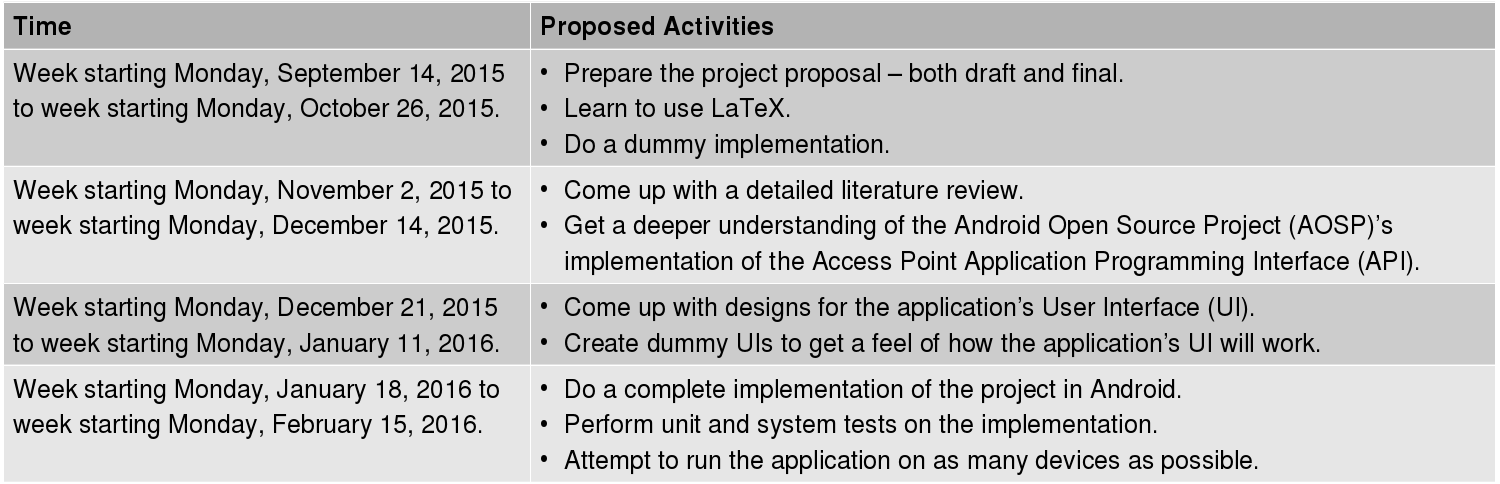
\includegraphics[width=\linewidth]{/run/media/joshua/DATA/ICS_2406_Pictures/00Proposal/Proposal_-_Schedule_Table}
	\caption{Proposed Project Schedule}
	\label{fig:Proposal:Proposed_Project_Schedule}
\end{figure}
% end figure proposed schedule table

%\begin{table} [ht]
%	\caption{Proposed Project Schedule}
%	\centering
%	\begin{tabular*}{\textwidth}{p{0.45\textwidth}|p{0.5\textwidth}}
%		\hline\hline
%		\\[-0.5ex]
%		\textbf{Time} & \textbf{Proposed Activities} \\[1ex]
%		\hline
%		\\[1ex]
%	
%		\raisebox{-0.5ex}{ \parbox{ 0.45\textwidth }{Week starting Monday, September 14, 2015 \\
%												    to week starting Monday, October 26, 2015.} } & 
%						   \parbox{ 0.9\textwidth }  {
%							\begin{xitemize} 
%								\item Prepare the project proposal – both draft and final.
%								\item Learn to use LaTex.
%								\item Do a dummy implementation.
%							\end{xitemize} } \\
%
%		\\[1ex]
%		\hline
%		\\[1ex]
%		
%		\raisebox{-0.5ex}{ \parbox{ 0.45\textwidth }{Week starting Monday, November 2, 2015 \\
%													to week starting Monday, December 14, 2015.} } & 
%		                   \parbox{ 0.9\textwidth }  {
%							\begin{xitemize} 
%								\item Come up with a detailed literature review.
%								\item Get a deeper understanding of the Android Open Source Project (AOSP)’s implementation of the Access Point Application Programming Interface (API).
%							\end{xitemize} } \\
%		\\[1ex]
%		\hline
%		\\[1ex]
%
%		\raisebox{-0.5ex}{ \parbox{ 0.45\textwidth }{Week starting Monday, December 21, 2015 \\
%				to week starting Monday, January 11, 2016.} } & 
%		\parbox{ 0.9\textwidth }  {
%			\begin{xitemize} 
%				\item Come up with designs for the application’s User Interface (UI).
%				\item Design the application’s database.
%				\item Create dummy UIs to get a feel of how the application’s UI will work.
%				\item Come up with interfaces between the UI and the application’s database.
%			\end{xitemize} } \\
%			
%		\\[1ex]
%		\hline
%		\\[1ex]
%
%		\raisebox{-0.5ex}{ \parbox{ 0.45\textwidth }{Week starting Monday, January 18, 2016 \\
%				to week starting Monday, February 15, 2016.} } & 
%		\parbox{ 0.9\textwidth }  {
%			\begin{xitemize} 
%				\item Do a complete implementation of the project in Android.
%				\item Perform unit and system tests on the implementation.
%				\item Attempt to run the application on as many devices as possible.
%			\end{xitemize} } \\
%			
%			\\[1ex]
%			\hline
%	\end{tabular*}
%	\label{table:schedule}
%\end{table}

% end Schedule
% ============

% begin Budget
% ============

\section{ \textbf{ Budget } } 

I roughly estimate that I will need the following resources to achieve the desired objectives of this project:

\begin{itemize}
	\item \textbf{10 GB worth of Safaricom data bundles.} The bundles will be used to access relevant information in the Internet. As of Sunday, 25 October 2015, Safaricom sells 3 GB worth of data for 30 days at Kshs. 1,000. 10 GB worth of data will call for the purchase of at least four sets of the 3 GB offer, resulting in 12 GB worth of data. Four sets of 3 GB bundles will cost Kshs. 4,000.
\end{itemize}

As of Sunday, 25 October 2015, the estimated amount needed for this project is Kshs. 4,000.

% end Budget
% ==========

% begin Other Information
% =======================

\section{ \textbf{ Other Information } } 

As of Sunday, 25 October 2015 there is no information to put in this section.

% end Other Information
% =====================

% begin Conclusion
% ================

\section{ \textbf{ Conclusion } } 

The proposal presented above is a light one. It serves as an introduction to what this project aims to do. It is hoped that this proposal will act as a guide during the next few months and will assist in the conversion of the project idea to an actual software system.

% end Conclusion
% ==============

% begin References
% ================

\newpage
\begin{thebibliography}{ 10 }
% The 10 implies you will add upto 10 references. You can 1ncrease this number if you have more than this number.

\bibitem{ Arul13 }

Arul Oli, V. C. K. P., 2013, 'Wireless Fidelity Real Time Security System', \emph{International Journal of Computer Science Trends and Technology},	vol. 1, no. 1, pp. 43-50, viewed Saturday, October 24, 2015, http://arxiv.org/ftp/arxiv/papers/1405/1405.1019.pdf

\bibitem{ Beck08 }

Beck, J., and Grajeda, T., 2008,
\emph{Lowering the Boom: Critical Studies in Film Sound}, p. 43, University of Illinois Press, Champaign, IL, USA. 

\bibitem{ Deitel12 }

Deitel, P., Deitel, H., Deitel, A., and Morgano, M. 2012, \emph{Android for Programmers An App-Driven Approach}, Pearsion Education, Inc., Crawfordsville, IN, USA.

\bibitem{ Ibn12 }

Ibn Minar, N. B., and Tarique, M., 2012, 'Bluetooth Security Threats ans Solutions: A Survey', \emph{International Journal of Distributed and Parallel Systems (IJDPS)} , vol. 3, no. 1, pp. 127-148, viewed Saturday, October 24, 2015, http://www.airccse.org/journal/ijdps/papers/0112ijdps10.pdf

\bibitem{ Preethi12 }

Preethi, K., Sinha, A., and Varma, N., 2012, 'Contactless Communication through Near Field Communication', \emph{International Journal of Advanced Research in Computer Science and Software Engineering}, pp. 158-163, viewed Saturday, October 24, 2015, http://www.ijarcsse.com/docs/papers/April2012/Volume\_2\_issue\_4/V2I40047.pdf

\bibitem{ Singh11 }

Singh, P., Sharma, D., and Agrawal, S., 2011, 'A Modern Study of Bluetooth Wireless Technology', \emph{International Journal of Computer Science, Engineering and Information Technology}, vol. 1, no. 3, pp. 55-63, viewed Saturday, October 24, 2015, http://airccse.org/journal/ijcseit/papers/0811ijcseit06.pdf

\bibitem{ Skariah13 }

Skariah, M., and Suriyakala, C. D., 2013, 'An Exploration on Wi-Fi/802.11b and WiMAX/802.16 Networks with Performance Enhancements', \emph{International Journal of Engineering Sciences and Research Technology}, vol. 2, no. 12, pp. 3658-3664, viewed on Sunday, October 25, 2015, http://www.ijesrt.com/issues\%20pdf\%20file/Archives\%202013/dec-2013/71.pdf

\bibitem{ Song14 } 

Song, S., and Isaac, B., 2014, 'Analysis of Wi-Fi and WIMAX and Wireless Network Coexistence', \emph{International Journal of Computer Networks and Communications (IJCNC)}, vol. 6, no. 6, pp. 63-78, viewed on Sunday, October 25, 2015, http://www.ijesrt.com/issues\%20pdf\%20file/Archives\%202013/dec-2013/71.pdf


\end{thebibliography}

% end References
% ================

\end{document}


























